\documentclass[../main.tex]{subfiles}

\begin{document}

\begin{workout}[tecniche Doppler vs fotometriche]
Si osservano fenomeni periodici, tramite tecniche fotometriche o spettroscopiche, tramite effetto doppler
\end{workout}

\begin{workout}[Periodo oscillazione-struttura interna]
 in numerose regioni del diagramma di \hr{}: l'osservazione di fenomeni periodici nelle stelle permette di dedurre informazione sulla loro struttura interna
\end{workout}

\begin{workout}[Spazio parametri modello stellare]
  di ridurre le incertezze nello spazio dei parametri del modello stellare.
\end{workout}

Le stelle in sequenza principale, come il Sole nella fase attuale, sono caratterizzate da numerosi modi di oscillazione di piccola ampiezza: onde gravo-acustiche stazionarie le cui caratteristiche sono determinate dal profilo radiale di $P$ e $\rho$, dal profilo radiale della velocit\'a del suono: le frequenze delle oscillazioni sono determinate principalmente dalla stratificazione e dinamica della regione in cui le ampiezze delle oscillazioni sono apprezzabili. Lo studio delle oscillazioni della superficie solare e l'estrapolazione delle informazioni sulla struttura interna in esse contenuta \'e detta eliosismologia.

In questa sezione ricavo l'equazione del moto perturbato che descrive i modi normali del Sole: considero piccole perturbazioni dello stato di equilibrio e adiabatiche cio\'e molto pi\'u rapide del tempo scala per scambio di calore dovuto al flusso radiativo o alle reazioni nucleari.

Le frequenze delle oscillazioni adiabatiche sono determinate dalla struttura interna del Sole attraverso i coefficienti che compaiono nelle equazioni che descrivono i modi normali: dato che $P,\ \rho,\ g$ non sono indipendenti \'e sufficiente specificare $\rho(r)$ e $\Gamma_1(r)$.


{\let\clearpage\relax\let\cleardoublepage\relax
\chapter{Modi normali.}
}

\section{Perturbazione dello stato di equilibrio.}

Descrivo le oscillazioni come piccole perturbazioni attorno allo stato di equilibrio stazionario (gli effetti non lineari, fra cui lo scambio di energia tra i modi, sono dell'ordine di $\frac{v}{c_s}$ dove v \'e l'ampiezza della velocit\'a dell'oscillazione). Indico con $P'(\vec{r},t)$ e $\delta P$ la perturbazione euleriana e lagrangiana della pressione e con $\rho'$, $\Phi'$ e $\vec{g}'$ la perturbazione euleriana della densit\'a , e le perturbazioni euleriane del potenziale gravitazionale e dell'accelerazione di gravit\'a conseguenti,  con $\delta\vec{r}=\vec{\xi}$ il vettore spostamento perturbato e con $\vec{v}=\PDof{t}(\Lvar{\vec{r}})$ la sua  velocit\'a:
\begin{align}
&P(\vec{r},t)=P_0(\vec{r})+P'(\vec{r},t)\label{eq:pressureperturbation}\\
&\Lvar{P(\vec{r})}=P(\vec{r}+\Lvar{\vec{r}})-P_0(\vec{r})=P'(\vec{r})+\Lvar{\vec{r}}\cdot\nabla P_0\\
&\vec{g}'=-\nabla\Phi',\ \nabla^2\Phi'=4\pi G\rho'\label{eq:gapert}
\end{align}

Ricavo l'equazione del moto perturbato sostituendo \eqref{eq:pressureperturbation} nell'equazione del moto \eqref{eq:motion} considerando solo i termini lineari nella perturbazione:
\begin{align}
&\rho\TDof{t}v\indices{_i}=\rho(\PDy{t}{v\indices{_i}}+v\indices{_j}\partial\indices{_j}v\indices{_i})=-\partial\indices{_i} P+\rho\vec{g}\indices{_i}\\
&\rho_0\PtwoDy{t}{\Lvar{\vec{r}}}=\rho_0\PDy{t}{\vec{v}}=-\nabla P'+\rho_0\vec{g}'+\rho'\vec{g}_0\label{eq:emper}
\end{align}

Analogamente per l'equazione di continuit\'a ottengo
\begin{equation}
\rho'+\div{(\rho_0\Lvar{\vec{r}})}=0\label{eq:contper}
\end{equation}


\section{Oscillazioni lineari adiabatiche.}

Considero i tempi caratteristici per scambio di calore per un elemento di fluido soggetto a un moto periodico: sono molto maggiori del periodo delle pulsazioni solari.

L'equazione di conservazione dell'energia interna \eqref{eq:primatemp}, esplicitando il bilancio di calore \eqref{eq:heatgl}, \'e

\begin{equation}
\TDy{t}{T}-\frac{\Gamma_2-1}{\Gamma_2}\frac{T}{P}\TDy{t}{P}=\frac{1}{c_P}(\epsilon-\frac{1}{\rho}\scap{\nabla}{F})
\end{equation}

Stimo il tempo caratteristico $\tau_R$ per flusso radiativo \eqref{eq:radfluxTgradrelation}, con $H$ lunghezza caratteristica per  la variazione di T:

\noindent
\begin{minipage}[c]{0.5\textwidth}
\begin{align*}
&\frac{1}{\rho c_P}\nabla\cdot(\frac{4acT^3}{3\kappa\rho}\nabla T)\approx\frac{4acT^4}{3\kappa\rho^2c_PH^2}=\frac{T}{\tau_R}\\
&\tau_R=\num{e12}\frac{\kappa\rho^2H^2}{T^3}\ (\si{\cgs})
\end{align*}
\end{minipage}
\begin{minipage}[c]{0.5\textwidth}
\begin{tabular}{ll}
Sole&Zona convettiva\\
$\tau_R\approx\SI{e7}{\year}\approx\tkh{}$&$\tau_R\approx\SI{e3}{\year}$\\
\end{tabular}
\end{minipage}

%Sole: $\kappa=1$, $\rho=1$, $T=\num{e6}$, $H=\num{e10}$)
%Zona convettiva$\kappa=100$, $\rho=\num{e-5}$, $T=\num{e4}$, $H=\num{e9}$)

Nella parte interna il termine dovuto alle reazioni nucleari \'e caratterizzato da un tempo $\tau_{\epsilon}\approx\frac{c_PT}{\epsilon}\approx\tkh{}$.

Confronto $\frac{T}{\tau_R}$, $\frac{T}{\tau_{\epsilon}}$ con $\TDy{t}{T}\approx\frac{T}{\Pi_{osc}}$ con $\Pi_{osc}\approx\si{\minute}-\si{\hour}$: i termini dovuti allo scambio di calore sono trascurabili. L'approssimazione adiabatica non \'e pi\'u valida vicino alla superficie solare dove i tempi per lo scambio di calore sono pi\'u brevi.

Il moto di una elemento di fluido \'e descritto dalla relazione adiabatica
\begin{equation}
\TDy{t}{P}=\frac{\Gamma_1P}{\rho}\TDy{t}{\rho}
\end{equation}

\begin{wrapfigure}[23]{r}{0.5\textwidth}
\centering
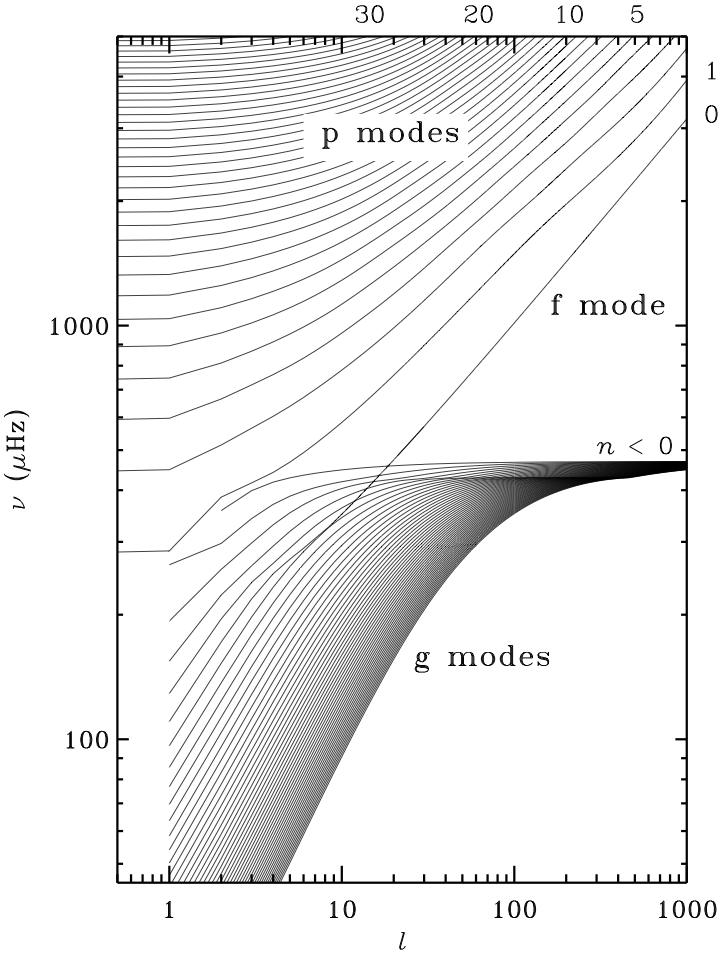
\includegraphics[keepaspectratio,width=0.45\textwidth]{nrmodesLAWE}
\caption{Modi adiabatici calcolati sulla base di un modello solare. Da \cite{chr02helioseismology}.}\label{fig:nrmodesLAWE}
\end{wrapfigure}

La condizione di perturbazione adiabatica linearizzata \'e
\begin{align}
&\PDy{t}{\Lvar{P}}-\frac{\Gamma_{1,0}P_0}{\rho_0}\PDy{t}{\Lvar{\rho}}=0\nonumber&\intertext{che integrata rispetto a t ed in funzione della variazione euleriana diventa}\\
&P'+\Lvar{\vec{\xi}}\cdot\nabla P_0=\frac{\Gamma_{1,0}P_0}{\rho}(\rho'+\Lvar{\vec{\xi}}\cdot\nabla\rho_0)\label{eq:adper}
\end{align}

\begin{workoput}[Propriet\'a armoniche sferiche]
Descrivo la dipendenza temporale dei modi normali tramite $\exp{i\omega t}$ e angolare tramite le funzioni armoniche sferiche $Y_{lm}(\theta,\phi)$;
\end{workout}

 inoltre, introducendo la frequenza di \bv{} (vedi \eqref{eq:bvfs}), $a=\Phi'+\frac{P}{\rho_0}$, $b=\div{\vec{\xi}}$, riscrivo l'equazione del moto \eqref{eq:emper} nella forma (vedi \citet*{ledoux1958variable})
\begin{align}
&\omega^2\vec{\xi}=\nabla a+\frac{N^2c^2}{g}b\frac{\vec{r}}{r}\\
&\hat{r}\cdot(\rot{\vec{\xi}})=0\ \Rightarrow\ \PDof{\theta}(\sin{\theta}\xi_{\phi})-\PDy{\phi}{\xi_{\theta}}=0
\end{align}
\'E quindi possibile ricavare la componente tangenziale della perturbazione da una funzione scalare:
\begin{equation}
\vec{\xi}=\exp{i\omega t}(\xi_r(r),\xi_h(r)\PDof{\theta},\frac{\xi_h(r)}{\sin{\theta}}\PDof{\phi})Y_l^m(\theta,\phi)
\end{equation}
dove ho scomposto il vettore spostamento perturbato in componente radiale $\xi_r(r)$ e tangenziale $\xi_h(r)$.



La variazione euleriana di densit\'a, pressione, potenziale gravitazionale sono espresse
\begin{equation}
(\rho',P',\Phi')=\exp{i\omega t}[\rho'(r),P'(r),\Phi'(r)]Y_l^m
\end{equation}
quindi ricavo la componente $\xi_h(r)$ applicando la parte tangenziale della divergenza all'equazione del moto:
\begin{equation}
\xi_h(r)=\frac{L}{r\omega^2}(\frac{P'(r)}{\rho_0}+\Phi'(r))
\end{equation}

mentre per $\xi_r(r)$:
\begin{align}
&\frac{1}{r^2}\TDof{r}(r^2\xi_r)-\frac{\xi_rg}{c^2}+\frac{1}{\rho_0}(\frac{1}{c^2}-\frac{l(l+1)}{r^2\omega^2})P'-\frac{l(l+1)}{r^2\omega^2}\Phi'=0\nonumber\\
&\frac{1}{\rho_0}(\TDof{r}+\frac{g}{c^2})P'-(\omega^2-N^2)\xi_r+\TDy{r}{\Phi'}=0\label{eq:eigenomega}\\
&\frac{1}{r^2}\TDof{r}(r^2\TDy{r}{\Phi'})-\frac{l(l+1)}{r^2}\Phi'-\frac{4\pi G\rho_0}{g}N^2\xi_r-\frac{4\pi G}{c^2}P'=0\nonumber
\end{align}

con $g=-\frac{1}{\rho_0}\TDy{r}{P_0}$.

Il sistema di equazione \eqref{eq:eigenomega} ha soluzione con le opportune condizioni al contorno per un insieme discreto di valori delle frequenze, $\omega_{nlm}$. L'ordine angolare m non compare nelle equazioni quindi gli autovalori $\omega_{nlm}$ sono $2l+1$ degeneri: la degenerazione \'e rimossa nel caso si tenga conto della rotazione ($\frac{\Omega}{\omega}\approx\num{e-4}$) o di effetti gravitazionali di altri corpi.

Condizioni al contorno: sono necessarie 4 condizioni.
\begin{itemize}
\item Due condizioni per $r=0$ selezionano le soluzioni regolari:
\begin{equation}
P'=0,\ \Phi'=0
\end{equation}
Vicino a zero risulta un andamento asintotico
\begin{equation}
(l\neq0):\ \xi_r\propto r\expy{l-1};\ (l=0):\ \xi_r\propto r;P',\ \Phi'\propto r^l
\end{equation}

\item Alla superficie solare richiediamo la continuit\'a di $\Lvar{\nabla\Phi}$ e che non si abbia propagazione verso l'esterno.
All'esterno della stella ho $\rho'=0$ quindi scelgo la soluzione nulla a infinito dell'equazione di Poisson $\Phi'=Ar\expy{-l-1}$:
\begin{equation}
\TDy{r}{\Phi'}+\frac{l+1}{r}\Phi'=0,\ r=\rsun{}    
\end{equation}
La condizione di non propagazione oltre la fotosfera dipende dalla descrizione dell'atmosfera solare. Nella versione pi\'u semplice impongo che la variazione di pressione sia zero alla superficie perturbata della stella
\begin{align}
&\Lvar{P}=P'+\xi_r\TDy{r}{P}=0
\end{align}
\end{itemize}

\begin{workout}[normalizzazione]

\begin{equation}
\omega_{\alpha}^2\int d^3x\rho|\vec{\xi}_{\alpha}(\vec{x})|^2=1
\end{equation}

vedi libbrecht88 figura power/gamma/E delle oscillazioni

\end{workout}


\begin{workout}[Discrepanze frequenze teoriche vs osservate]

[nFreqdiff]

Per distinguere gli effetti dovuti alla non corretta descrizione fisica dei modi vicino alla superficie, $r>0.95\rsun{}$, cui sono pi\'u sensibili i modi di l elevato, si introduce
\begin{equation}
Q_{nl}=\frac{E_{nl}}{E^0_{nl}}\label{eq:surfaceeffects}
\end{equation}
che vale 1 per $l=0$ e diminuisce al crescere di $l$.

%[figura dalsgaard 2002 fig deltanu/deltanu]

 e definisco l'inerzia del modo
\begin{equation}
I_{nl}=\int d^3x\rho_0(\vec{\xi}^*\cdot\vec{\xi})\label{eq:modeinertia}
\end{equation}

$Q_{nl}=I_{nl}/I_{0}(\omega_{nl})$

\end{workout}



{\let\clearpage\relax\let\cleardoublepage\relax
\chapter{Analisi del campo di velocit\'a della superficie solare.}
}


\section{Identificazione fenomeni periodici}

\begin{workout}[altezze linee assorbimento metalli]
[Tabella 1 \cite{houdek2006stochastic}.]
perch\'e? Diminuzione T formazione atomo? Diminuzione pressione minori collisioni?
\end{workout}



Una parte basilare dell'informazione contenuta nei modi di oscillazione \'e ricavata analizzando  lo spostamento doppler delle righe di assorbimento dei metalli presenti negli strati visibili pi\'u esterni del sole.

L'ampiezza della velocit\'a di oscillazione per il singolo modo \'e  al pi\'u \SI{15}{\cm\per\second} quindi l'effetto doppler causa uno shift, al massimo, di $\frac{\Delta\lambda}{\lambda}\approx\num{e-10}$: tale shift si pu\'o misurare attraverso uno spettroscopio a scattering risonante  , per misure senza risoluzione spaziale, o con un tacometro di Fourier dove \'e necessaria risoluzione spaziale.

% Na $D$ lines: $\lambda=\SI{589.6}{\nano\meter},\SI{589.0}{\nano\meter}$; SOHO (MDI): Ni \SI{678.8}{\nano\meter}; K Fraunhofer line \SI{770}{\nano\meter}; Ca \SI{643.9}{\nano\meter}; K \SI{769.9}{\nano\meter}


Per identificare i modi di oscillazione non radiali \'e necessario considerare anche la dipendenza spaziale del campo di velocit\'a per ottenere, tramite trasformata di Fourier, lo spettro di potenza.

Un segnale di durata T permette una risoluzione $\Delta\omega=\frac{2\pi}{T}$: se devo risolvere due frequenze $\omega$ e $\omega+\Delta\omega$ devo osservare per un tempo $T=\frac{2\pi}{\Delta\omega}$ e la frequenza pi\'u bassa osservabile \'e $\Delta\omega$. Il limite superiore delle frequenze osservate \'e dato dalla frequenza di Nyquist $\omega_{Ny}=\frac{\pi}{\Delta t}$ con $\Delta t$ risoluzione temporale. Il dominio spazio-temporale quindi definisce, con analoghe relazioni per le variabili spaziali cartesiane e vettore d'onda associato, il dominio nello spazio $(\omega,\vec{k}_h)$ con $\vec{k}_h=(k_x,k_y)$
\begin{equation}
\Delta\omega=\frac{2\pi}{T}\leq\omega\leq\frac{\pi}{\Delta t},\ \Delta k_i=\frac{2\pi}{L_i}\leq k_i\leq\frac{\pi}{\Delta x_i}
\end{equation}

In \citet{lei62velocity} si osserva che la superficie solare ha scale spazio-temporali privilegiate: in particolare \'e presente un comportamento periodico nell'atmosfera a tutte le altezze rilevato tramite effetto doppler. Il periodo \'e di circa 300 secondi e la lunghezza caratteristica di qualche \si{\mega\meter}.



\section{Onde stazionarie}

\begin{workout}[Deubner:ridge in $(k_h,\omega)$, Approx onda piana]

nell'approssimazione di onda piana si ha $k_h^2\approx\frac{l(l+1)}{r^2}$

Le osservazione del disco solare risolto spazialmente permettono di individuare i modi di alto grado angolare: l'analisi tramite FFT (frequenza e $k_h$) delle osservazioni della superficie solare riportate in \citet{deu75observations} ($CI\ \SI{538}{\nano\meter}$) confermano che la  potenza delle oscillazioni (con numero d'onda $k_h=\frac{2\pi}{\lambda}<\SI{1}{\per\mega\meter}$) si distribuisce in linee determinate nel diagramma $(k_h,\omega)$ predette dal modello e quindi conferma che sono provocate da modi acustici non radiali degli strati interni alla fotosfera.

Segnale doppler periodico: $k_h=\sqrt{k_x^2+k_y^2}$ numero d'onda orizzontale e $\vec{k}=k_r\hat{r}+\vec{k}_h$:  i modi si concentrano in determinate regioni del diagramma  $(k_h,\omega)$.
\end{workout}

\begin{workout}[Proiezioni $V_D$ su armoniche sferiche]
La simmetria sferica del modello solare rende naturale una descrizione delle perturbazioni in funzione di $Y\indices{_l^m}(\theta,\phi)$, l \'e l'ordine angolare. Le funzioni armoniche sferiche  soddisfano
\begin{equation}
L^2Y_l^m=-\frac{1}{\sin{\theta}}\PDof{\theta}(\sin{\theta}\PDy{\theta}{Y_l^m})+\frac{1}{\sin^2{\theta}}\PtwoDy{\phi}{Y_l^m}=-r^2\nabla_h^2Y_l^m=l(l+1)Y_l^m\label{eq:SHperturb}
\end{equation}


Considero la geometria sfrerica descrivendo la dipendenza spaziale tramite le funzioni armoniche sferiche con l'asse delle sul piano del cielo ortogonale alla linea di vista. Il segnale Doppler osservato \'e proporzionale a:
\begin{equation}
    V_D(\theta,\phi,t)=\sin{\theta}\cos{\phi}\sum_{n,l,m}A_{nlm}c_{lm}P_l^m(\cos{\theta})\cos{(m\phi-\omega_{nlm}t-\beta_{nlm})}
\end{equation}

\end{workout}

Il fattore $\sin{\theta}\cos{\phi}$ deriva dalla proiezione della velocit\'a radiale sulla linea di vista: i modi relativi alle oscillazioni dei 5 minuti di grado l non elevato causano uno spostamento quasi totalmente radiale.

Per isolare il contributo di una singola $Y_{l_0m_0}$ considero
\begin{equation}
V_{l_0m_0}(t)=\int_AV_D(\theta,\phi,t)W_{l_0m_0}(\theta,\phi)\,dA=\sum_{n,l,m}S_{l_0m_0,lm}A_{nlm}(t)\cos{(\omega_{nlm}t+\beta_{nlm,L_0m_0})}
\end{equation}
e ho integrato sul disco solare con $W_{l_0m_0}\approx Y_{l_0m_0}$. La funzione di risposta $S_{l_0m_0,lm}\propto\delta_{ll_0}\delta_{mm_0}$ poich\'e le armoniche sferiche sono ortogonali sull'intera sfera $V_{l_0m_0}(t)$ contiene contributi da valori di $(l,m)$ vicini.

\begin{workout}[Power spectral density]
La trasformata di Fourier di $V_{l_0m_0}(t)$ permette di isolare i modi come picchi nello spettro di potenza:
\begin{equation}
P(\omega,l,m)=|A_{nlm}|^2(\omega)
\end{equation}

Random precess x(t) sampled over finite window time T:
\begin{align}
&S_T(\nu)=\frac{1}{T}|X_T(\nu)|^2\\
&S_T(\nu)=\frac{1}{T}\int_{-T/2}^{T/2}\int_{-T/2}^{T/2}x(t)x(t')\exp{i2\pi\nu t}\exp{i2\pi\nu t}\,dt\,dt'\\
&=S_T(\nu)=\int_{-T/2}^{T/2}\left[\frac{1}{T}\int_{-T/2}^{T/2}x(t')x(t'+\tau)\,dt'\right]\exp{i2\pi\nu \tau}\,d\tau\\
&S_T(\nu)=\int_{-T/2}^{T/2}C_T(\tau)\exp{i2\pi\nu\tau}\,d\tau\\
&C(\tau)=E(x(t)x(t+\tau))=\lim{T\to\infty}C_T(\tau)&\intertext{Introduco la densit\'a spettrale $S_x(\nu)$:}\nonumber\\
&S_x(\nu)=\lim{T\to\infty}E[S_T(\nu)]=\int_{-\infty}^{-\infty}C(\tau)\exp{2\pi i\nu\tau}\,d\tau&\intertext{Wiener-Khinchin theorem}\nonumber\\
&C(\tau)=\int_{-\infty}^{-\infty}S_x(\nu)\exp{-2\pi i\nu\tau}\,d\nu\nonumber\\
&C(0)=\int_{-\infty}^{-\infty}S_x(\nu)\,d\nu=E(x^2)&\intertex{Parseval's theorem}
\end{align}
\end{workout}

Il modello proposto da \citet{ulrich70five} e \citet*{stein71five} considera le propriet\'a dei modi normali non radiali di oscillazione del Sole, in particolare usando la relazione di dispersione per onde acustiche, si ha la definizione di cavit\'a risonanti all'interno del Sole: la variazione delle propriet\'a del gas delimita le regioni di propagazione a diverse profondit\'a a seconda delle caratteristiche trasversali del moto.

\begin{workout}[Modi nodi]
L'andamento di un modo sulla superficie solare determina $(l,m)$ mentre l'ordine radiale n si ricava dalla distribuzione delle frequenze di oscillazione.
\end{workout}

\begin{workout}[Mode mass and height of line]
Relazione tra power of modes at surface and total energy of the mode
\end{workout}

\section{Misura splitting in m}

\begin{workout}[fitting power spectra to measure splitting coefficients]
Le deviazioni dalla simmetria sferica causano uno splitting delle frequenze: rappresento un multipletto di frequenze tramite espansione con base di polinomi appropriata (solitamente si usano i polinomi di Legendre)
\begin{equation}
\nu_{nlm}=\nu_{nl0}+\sum_{j=1}^{j_{\max}}a_j(n,l)\pol_j^{(l)}(m)\label{eq:freqmulti}
\end{equation}
e ricavo i coefficienti tramite fit con le frequenze osservate; i coefficienti dispari contengono il contributo della rotazione al termine lineare, i coefficienti pari effetti delle asfericit\'a nella struttura solare e effetti quadratici della rotazione.

Media su m vs $m=0$ o $m=l$
\end{workout}


\begin{workout}[Departure from spherical symmetry lift the (2l+1)-fold degeneracy]

Deviazioni dalla simmetria sferica introducono una dipendenza delle frequenze dei modi da m. L'effetto della rotazione \'e descritto al primo ordine (in $\Omega$) da 
\begin{equation}
\Delta\omega_{nlm}
\end{equation}

Spesso \'e impossibile misurare lo splitting in m quindi si parametrizzano le frequenze nel multipletto $(n,l)$ tramite:
\begin{equation}
\nu_{nlm}=\nu_{nl0}+\sum_{j=1}^{j_{\max}}a_j(n,l)\pol_j^{(l)}(m)\label{eq:freqmulti}
\end{equation}


\end{workout}


Le oscillazioni osservate hanno $\nu\geq\SI{500}{\micro\hertz}$, sono causate da modi p, onde stazionarie che si propagano come onda evanascente nell'atmosfera solare, e modi f, onde di superficie, di alto grado l.


Le osservazioni della luce integrata sull'intero disco selezionano modi di basso grado angolare: \citet{cla79solar} osservano nello spettro Doppler (linee di assorbimento di K neutro: \SI{769.9}{\nano\meter}) della luce integrata sull'intero disco solare dei picchi equi-spaziati circa \SI{68}{\micro\hertz} interpretate come modi p di alto ordine n e basso grado l. I modi di basso ordine radiale l penetrano in profondit\'a e quindi portano informazioni sulle regioni di fusione e la loro evoluzione.


\begin{workout}[Osservazioni low-high degree attuali]

\begin{wrapfigure}[6]{r}{0.6\textwidth}
\centering
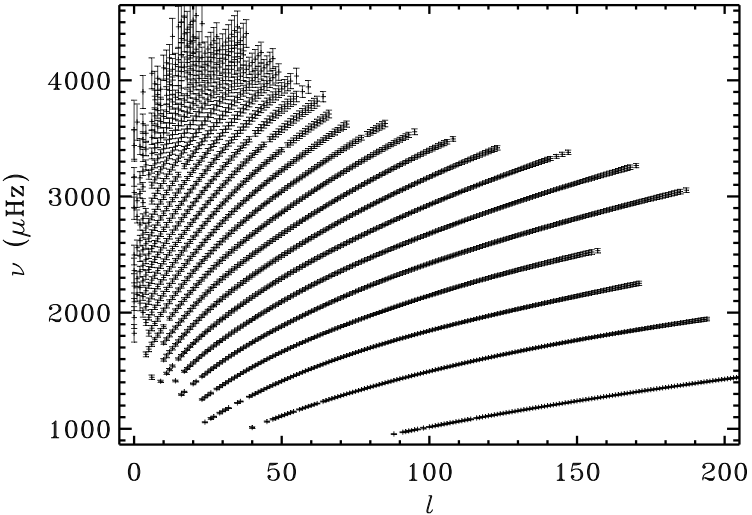
\includegraphics[keepaspectratio,width=0.45\textwidth]{midlmodes}
\caption{Distribuzione dei modi con $l\leq300$ nel diagramma $\nu-l$. Da \cite{chr02helioseismology}.}\label{fig:midlmodes}
\end{wrapfigure}

\begin{wrapfigure}[6]{r}{0.6\textwidth}
\centering
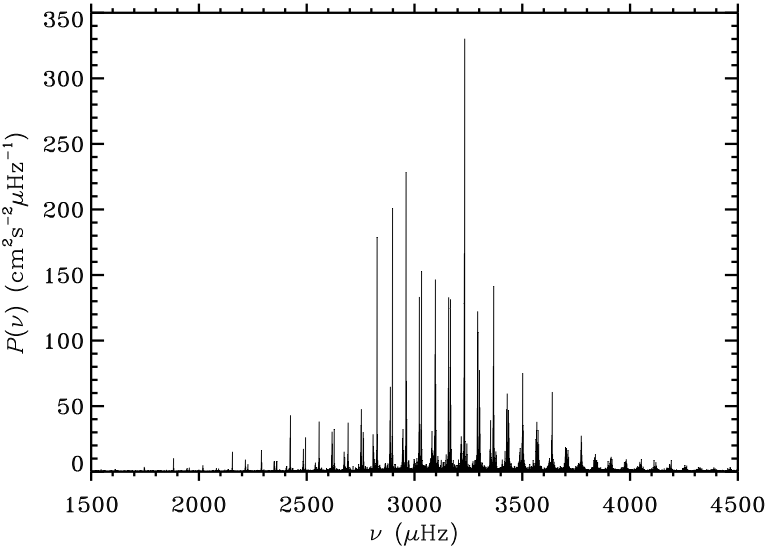
\includegraphics[keepaspectratio,width=0.45\textwidth]{lowlmodes}
\caption{Spettro modi di basso grado angolare. Da \cite{chr02helioseismology}.}\label{fig:lowlmodes}
\end{wrapfigure}

\end{workout}


{\let\clearpage\relax\let\cleardoublepage\relax
\chapter{Eccitazione e tempo di vita dei modi.} \label{chap:excitation}
}

\begin{workout}[Ampiezza dei modi]



\end{workout}

\begin{workout}[Convoluzione source e funzione risposta]
Modelling solar oscillation power spectra (ADH90): formula 2 ??
\end{workout}


\begin{workout}[Energia totale del modo]

\begin{equation}
E_{tot}=\int_0^M\,dm\exv{\dot{\xi}^2}=\frac{1}{2}\exv{|A|^2}I\omega_0^2, \ I=\int\,d^3x\rho_0(\vec{\xi}*\vec{\xi})
\end{equation}

\end{workout}

\begin{wrapfigure}[23]{r}{0.5\textwidth}
\centering
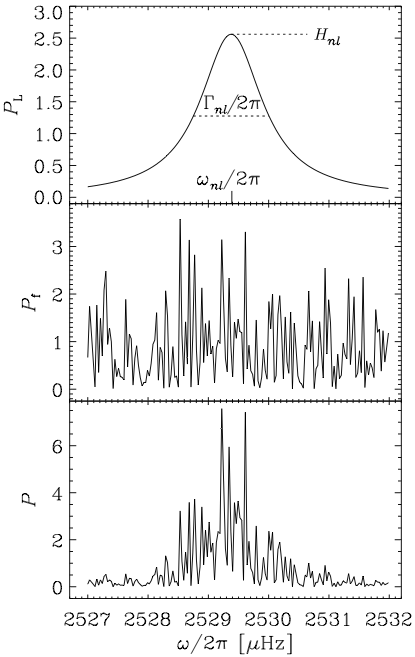
\includegraphics[keepaspectratio,width=0.4\textwidth]{Powerspectraldensity}
\caption{$\exv{P}=|A(\omega)|^2$ spettro di oscillatore armonico forzato, smorzato di frequenza naturale $\midfrac{\omega_{nl}}{2\pi}$. Da \cite{houdek2006stochastic}.}\label{fig:Powerspectraldensity}
\end{wrapfigure}

Un modello per l'eccitatazione dei modi p alle ampiezze osservate descrive l'interazione tra i modi e i moti turbolenti dovuti alla convezione tramite un insieme di oscillatori smorzati di frequenze naturali $\omega_{nl}$ e sottoposti a forzante stocastica: trascuro gli effetti non lineari e eventuali instabilit\'a intrinche alle pulsazioni.

\begin{equation}
I_{nl}[\TtwoDy{t}{\xi_{nl}}+\Gamma_{nl}\TDy{t}{\xi_{nl}}+\omega_0^2\xi_{nl}]=f(t)
\end{equation}

con $\xi_{nl}$ ampiezza dell'oscillatore, $\midfrac{\Gamma}{2}=\Im{\omega}$ costante di smorzamento.

La funzione $f(t)$ contiene il contributo dei moti turbolenti e fluttuazioni entropia causati dai moti convettivi.

Assumendo $\omega_{nl}\gg\Gamma_{nl}$, cio\'e gli scambi di energia tra i modi e la turbolenza hanno tempo caratteristico $\tau_{nad}\gg\Pi_{osc}$, lo spettro in frequenza dell'oscillatore $\exv{P(\omega)}=\exv{|\xi_{nl}(\omega)|^2}$ \'e della forma:
\begin{equation}
\exv{P(\omega)}\propto P_LP_f=\frac{\midfrac{\Gamma_{nl}}{2\pi}}{(\omega-\omega_0)^2+\midfrac{\Gamma_{nl}}{4}}P_f
\end{equation}

\begin{wrapfigure}[20]{r}{0.5\textwidth}
\centering
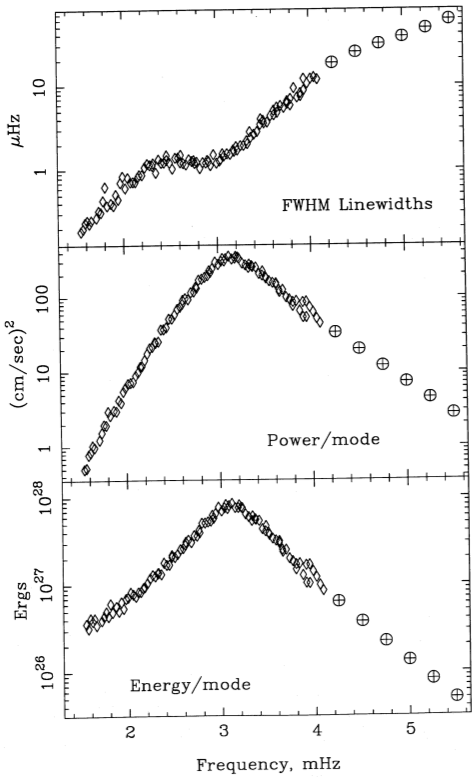
\includegraphics[keepaspectratio,width=0.4\textwidth]{modespheomenology}
\caption{FWHM per i modi osservati, $V_{nl}$, energia totale per modi con $l\approx20$. Da \cite{libbrecht1988solar}.}\label{fig:modespheomenology}
\end{wrapfigure}

La media temporale dell'energia di un modo \'e
\begin{align}
%E_{\omega_0}=\int_0^M\exv{v_{osc}^2}
&E_{nl}=I_{nl}V_{nl}^2\\
&=\frac{1}{2}I_{nl}\omega_{nl}\exv{|A_{nl}^2|}\propto I_{nl}\omega_{nl}\intsinf{}P(\omega)\,d\omega\\
&\propto\frac{P_f(\omega_{nl})}{\Gamma_{nl}}
\end{align}

\begin{align}
&H=\int_{\nu_0-\midfrac{\delta}{2}}^{\nu_0-\midfrac{\delta}{2}}|\tilde{V}(\nu)|^2\,d\nu\\
&H\approx\frac{2V_{rms}^2}{\eta}:\ T_{obs}\gg 2\tau\\
&H\approx V_{rms}^2T_{obs}:\ T_{obs}\ll 2\tau
\end{align}



[Si ipotizza che le oscillazioni siano eccitate in maniera stocastica dai moti convettivi: la larghezza delle frequenze risonanti \'e determinata dal tempo di smorzamento.]

[Extensive turbolent layers: stars lose all hint of vibrational instability]

[Not self excited: driven to observable amplitude by external process]

[Turbolent convection: source of pulsational energy, emit acustic radiation]

[Stable pulsation: spectrum as that of an ensemble of harmonic oscillator stocastically driven and damped]

[Power spectrum indipendent of l for $l<100$: low degree modes are not influenced by $k_h$. Vertical propagation: superficial layers (low l modes are generated in these strata)]


[Interaction with turbolent convection]

[Radiative transfer (as frequencies rise modes became more sensitive to rapid relaxation time in solar atmosphere)]

[La stabilit\'a dei modi g \'e determinata dalla stabilit\'a convettiva: se non sono presenti regioni di instabilit\'a convettiva i modi g sono stabili ($g_+$), se esistono zone convettivamente instabili esistono anche modi g instabili ($g_{\,-}$).]


[Excitation p-modes: fluctuating turbolent pressure (Raynold stresses). Excitation g-modes: nuclear burning instabilities. Damping: radiative losses, viscosity, nonlinear interaction between modes.]

[Low l p-modes exponential decay with e-folding time several days.]



{\let\clearpage\relax\let\cleardoublepage\relax           %%% Chapter  Caratteristiche asintotiche delle oscillazioni adiabatiche.
\chapter{Caratteristiche asintotiche delle oscillazioni adiabatiche.}\label{chap:asyntoticbehavour}
}


I modi gravo-acustici descritti in \eqref{eq:eigenomega} si riducono ai modi p ed f per alte frequenze e ai modi g per basse frequenze. Approssimando il comportamento della perturbazione localmente con un'onda piana e trascurando la perturbazione al potenziale gravitazionale $\Phi'$ si ottendono soluzioni asintotiche per i modi normali e relazioni di dispersione approssimate.

\section{Comportamento asintotico.}

\begin{workout}[Equazioni oscillazioni adiabatiche: approssimazione di Cowling.]

Per determinare la struttura dello spettro delle oscillazioni introduciamo l'approssimazione di Cowling (\cite{cow41oscillations}) cio\'e trascuriamo la perturbazione del potenziale gravitazionale. Quindi il sistema \eqref{eq:eigenomega} si riduce al secondo ordine

\begin{subequations}\label{cowosc:main}
\begin{align}
&\frac{1}{r^2}\TDof{r}(r^2\xi_r)-\frac{\xi_rg}{c^2}+\frac{1}{\rho_0}(\frac{1}{c^2}-\frac{l(l+1)}{r^2\omega^2})P'=0\label{cowosc:a}\\
&\frac{1}{\rho_0}(\TDof{r}+\frac{g}{c^2})P'-(\omega^2-N^2)\xi_r=0\label{cowosc:b}
\end{align}
\end{subequations}

\end{workout}

\begin{workout}[Problema Sturm-Liuville: limite alte/basse frequenze]
Considero i limiti asintotici di alte e basse frequenze: ottengo un problema del tipo di Sturm-Liuville.
%https://en.wikipedia.org/wiki/Sturm%E2%80%93Liouville_theory
\begin{itemize}
\item Per $\omega\to\infty$: lo spettro \'e discreto, le oscillazioni sono prodotte da onde acustiche in cui la forza dominante \'e fornita dalla pressione, i modi p, ordinati in base al numero di zeri di $\xi_r$ fra il centro e la superficie.

\item Per $\omega\to0$ lo spettro \'e discreto, il moto \'e determinato dalla forza di gravit\'a: si hanno i modi g.

\end{itemize}
%Lo spettro solare \'e la combinazione dei modi parziali precedenti; 
I modi f separano i modi g e p: non hanno nodi in direzione radiale.
\end{workout}

\'E utile fare l'ulteriore approssimazione, valida per grandi n, di trascurare la variabile perturbata rispetto alla sua derivata radiale, e cos\'i si ottiene
\begin{equation}\label{eq:secondorder}
\TtwoDy{r}{\xi_r}=\frac{\omega^2}{c_s^2}(1-\frac{N^2}{\omega^2})(\frac{S_l^2}{\omega^2}-1)\xi_r=-K(r)\xi_r
\end{equation}
per $K(r)>0$ quest'equazione descrive un comportamento oscillante; considerando un'onda piana si ha la relazione di dispersione:
\begin{equation}
k_r^2=\frac{\omega^2}{c_s^2}(\frac{N^2}{\omega^2}-1)(\frac{S_l^2}{\omega^2}-1)\label{eq:approximatedispersion}
\end{equation}

\section{Cavit\'a risonanti.} \label{sec:resonantcavity} %Definizione frequenze critiche

I modi p e g sono confinati in regioni dell'interno solare determinate dalla variazione delle caratteristiche del plasma solare.
%La variazione delle propriet\'a del gas influenzano la velocit\'a del suono, $c_s=\Gamma_1\frac{P}{\rho}$, e le frequenze critiche: esistono regioni dell'interno solare, dipendenti dalla natura delle oscillazioni, in cui \'e possibile un comportamento periodico ai cui bordi si ha riflessione interna.

\begin{minipage}{\linewidth}
\begin{tikzpicture}
\node[inner sep=0pt] (image) at (-0.5,0)
  {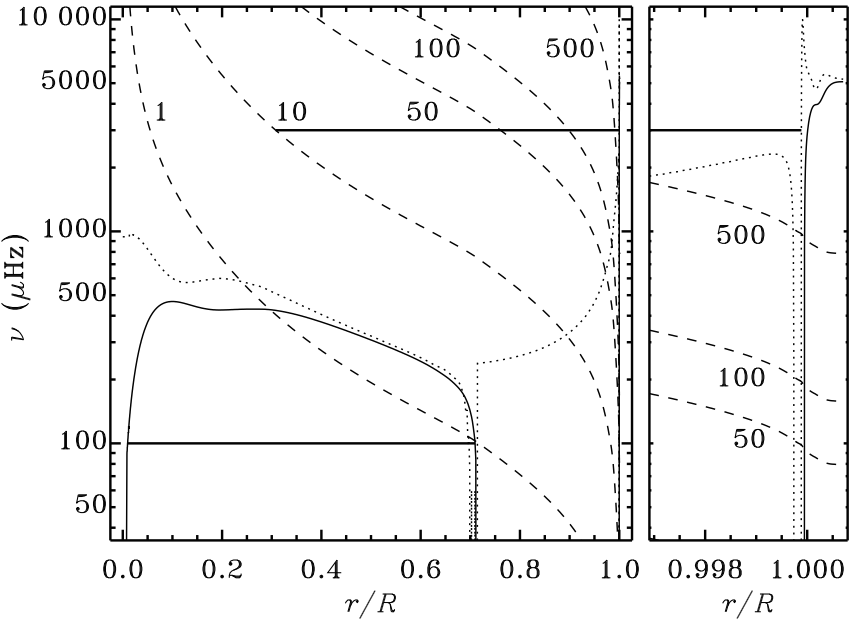
\includegraphics[keepaspectratio=true,scale=0.35]{cutoff}};
  \node (legenda) at (5.8,3) { Legenda };
  \draw [draw=black!50] (legenda.north west) rectangle +(0.35\textwidth, -4cm);
  \draw [dotted] (6,2) -- (5.5,2) node[at start, anchor=west] {$\frac{\omega_c}{2\pi}$;};
  \draw [dashed] (7.5,2) -- (7,2) node[at start, anchor=west] {$\frac{S_l}{2\pi}$;};
  \draw [] (9,2) -- (8.5,2) node[at start, anchor=west] {$\frac{N}{2\pi}$;};
  \node at (7.9,0.5) {\parbox{0.32\textwidth}{Le linee orizzontali a \SI{100}{\micro\hertz} e \SI{3000}{\micro\hertz} demarcano le regione in cui sono confinati risp. un modo g e p.}};
  \node (caption) at (7.6,-2.3) { \begin{minipage}[l]{0.3\textwidth}
\captionof{figure}{Frequenze caratteristiche calcolate tramite il modello S. Da \cite{chr02helioseismology}.\label{cutoff}}%   
    \end{minipage}};
\end{tikzpicture}
\end{minipage}

Le onde acustiche sono confinate in una regione che \'e limitata superiormente dall'aumento della frequenza critica acustica
\begin{equation}
\omega_A=\frac{c_s}{2\densityscale{}}\sqrt{1-2\TDy{r}{\densityscale{}}}\propto T\expy{-\frac{1}{2}}\label{eq:acusticcutoff}
\end{equation}
causato dalla diminuzione della temperatura che provoca la riflessione delle onde con periodo attorno ai 5-min, mentre l'aumento della velocit\'a del suono con la profondit\'a e la conseguente rifrazione dell'onda porta a propagazione del moto puramente tangenziale $k_r=0$ nel guscio sferico per cui $c_s=\frac{\omega}{k_h}\approx\omega \frac{r}{L}$ ovvero per $\omega=S_l$ frequenza di Lamb definita da
\begin{equation}
S_l^2=\frac{l(l+1)c_s^2}{r^2}\label{eq:Lambf}
\end{equation}

Maggiore \'e il grado l meno profonda \'e la cavit\'a: le cavit\'a acustiche si estendono nella zone convettiva fino alla profondit\'a in cui la rifrazione dovuta all'aumento della velocit\'a del suono $c_s\propto\sqrt{T}$ causa una riflessione totale dell'onda quando la velocit\'a del suono \'e aumentata fino alla loro velocit\'a di fase orizzontale.

%Si pu\'o stimare la profondit\'a della cavit\'a acustica, utilizzando la condizione $c_s=\frac{\omega}{k_h}$ per $k_r=0$: approssimo la temperatura al punto di inversione del moto con $T\approx\Dcvar{\TDy{r}{T}}{ad}\delta$ dove $\delta$ \'e la profondit\'a della cavit\'a e, ipotizzando un gas ideale, ho $\Dcvar{\TDy{r}{T}}{ad}=\frac{g}{c_P}$ con $c_P$ calore specifico a pressione costante per unit\'a di massa.
%Usando le relazioni fra gli esponenti adiabatici e che nel caso sono uguali a $\gamma$ riscrivo $c_s^2=(\Gamma_3-1)g\delta$ e sostituendo nella condizione al punto di inversione ottengo $\delta=\frac{\omega^2}{k_h^2(\Gamma_3-1)g}$: i modi con stesso $\frac{\omega}{k_h}$ sono confinati nella stessa cavit\'a.

%Le regione di propagazione dei modi g sono definite da $\omega<N$: i modi g sono confinati nelle regioni pi\'u interne del Sole.
Le onde di gravit\'a sono presenti nelle regioni in cui il gas \'e neutro o completamente ionizzato ($N^2$ grande) mentre sono riflesse dalle regioni dove $N$ \'e piccolo o immaginario: ionizzazione parziale, instabilit\'a convettiva, centro del Sole.
Ho cavit\'a risonanti per modi g:
\begin{itemize}
\item Core radiativo: i modi g sono confinati tra la la parte centrale dove $g\to0$ e il fondo della zona convettiva dove $N^2<0$.
\item Atmosfera: $N$ ha un massimo in coincidenza del punto $T_m$ nella cromosfera: modi g confinati tra zona convettiva e cromosfera ($\Pi\approx\numrange{180}{800}\si{\second}$).
\end{itemize}

\begin{figure}
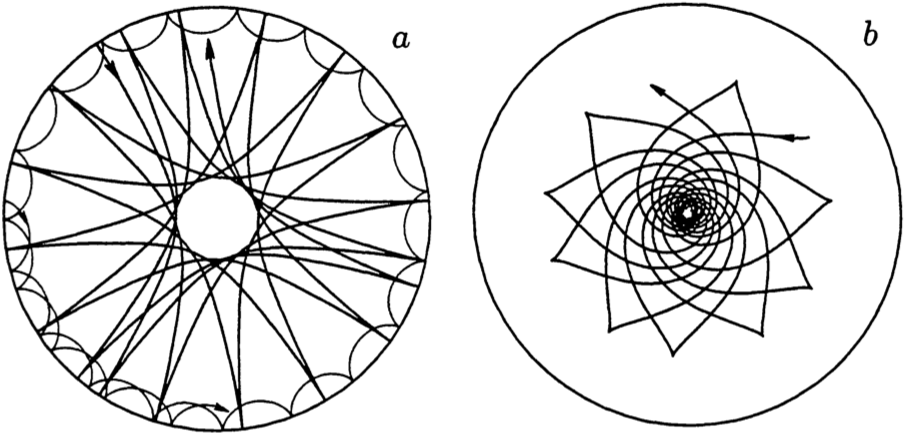
\includegraphics[keepaspectratio,width=0.8\textwidth]{raypath-gp}
\caption{(a): Percorso di due onda acustiche $p_8(l=2), p_8(l=100)$; (b): Percorso di un'onda di gravit\'a: $g_{10}(l=5)$. Da\cite{gou91seismic}.}
\end{figure}

\subsection{Condizione di risonanza radiale}
%[Specificare il valore di L: spherical harmonic expansion vs ray picture]

In \citet{duv82dispersion} si mostra che un grafico di $\frac{\pi(n+\alpha)}{\omega}$ rispetto a $\frac{\omega}{k_h}$ rappresenta i modi p con un'unica curva, per $\alpha$ opportuno, quindi:
\begin{equation}
(n+\alpha)\frac{\pi}{\omega}=F'(\frac{\omega}{k_h})=F(\frac{\omega}{L})\label{eq:duvallr}
\end{equation}

\begin{wrapfigure}[15]{r}{0.45\textwidth}
\centering
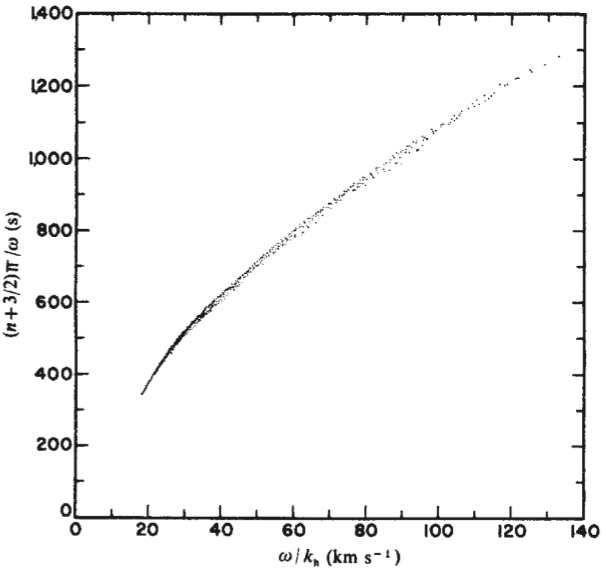
\includegraphics[keepaspectratio,width=0.4\textwidth]{dispersionDuvall}
\caption{I modi p sono rappresentati in un unica linea. Da \cite{duv82dispersion}.}
\end{wrapfigure}

Questo si giustifica considerando che, per l fissato, le frequenze dei modi sono determinate dalla condizione che l'onda interferisca costruttivamente con se stessa, come per una cavita chiusa ad un'estremit\'a. Un'onda stazionaria in direzione radiale implica che l'integrale di $k_r$ nella regione di propagazione fra due zeri consecutivi sia un intero multiplo di $\pi$ mentre $\alpha$ tiene conto del combiamento di fase nella riflessione.
\begin{equation}
(n+\alpha)\pi\approx\int_{r_t}^Rk_r\,dr\approx\int_{r_t}^R\frac{\omega}{c_s}\sqrt{1-\frac{S_l^2}{\omega^2}}\,dr\label{eq:duvallexpli}
\end{equation}
ho usato la relazione di dispersione per onde acustiche considerando il limite ad alte frequenze di \eqref{eq:approximatedispersion}
\begin{equation}
k_r^2\frac{\omega^2}{c_s^2}(\frac{S_l^2}{\omega^2}-1)
\end{equation}
quindi \'e
\begin{equation}
F(w)=\int_{r_t}^R\sqrt{1-\frac{c_s^2}{r^2w^2}}\,\frac{dr}{c_s}\label{eq:duvallf}
\end{equation}

Utilizzando invece il limite per basse frequenze di \eqref{eq:approximatedispersion} per i modi g trovo la relazione di dispersione approssimata per $l\neq0$

\begin{equation}
k_r^2=\frac{S_l^2}{c^2}(\frac{N^2}{\omega^2}-1)\label{eq:dispersionag}
\end{equation}
%[introdotta in precedenza \eqref{eq:bvf}]
e ottengo l'espressione analoga di \eqref{eq:duvallexpli} per i modi g
\begin{equation}
\frac{(n+\alpha_g)\pi}{L}\approx\int_{r_1}^{r_2}(\frac{N^2}{\omega^2}-1)\expy{\frac{1}{2}}\,d\ln{r}\label{eq:duvallg}
\end{equation}
con $r_2\approx R_{cz}$.

\subsection{Relazione di dispersione per i modi gravo-acustici.}

Approssimo il comportamento spaziale delle oscillazioni con quello di onda piana $\vec{\xi}\propto\exp{i\scap{k}{x}}$ con $\vec{k}=k_r\hat{r}+\vec{k}_h$.

Considero i coefficienti delle equazioni \eqref{cowosc:main} costanti ad eccezione di $P_0,\ \rho_0$: approssimazione valida se la lunghezza d'onda delle perturbazioni \'e molto minore della scala caratteristica di variazione dei coefficienti.
%stix local treatment pg 165

Sostituisco
\begin{align}
&\xi_r\propto\rho_0\expy{-\frac{1}{2}}\exp{ik_rr},\ P_1\propto\rho_0\expy{\frac{1}{2}}\exp{ik_rr}&\intertext{forma richiesta dalla conservazione dell'energia e della quantit\'a di moto, e ottengo la relazione di dispersione}\nonumber\\
&k_r^2=\frac{\omega^2-\omega_A^2}{c^2}+S_l\frac{N^2-\omega^2}{c^2\omega^2}=\frac{\omega^2}{c^2}(1-\frac{\omega_{l,+}^2}{\omega^2})(1-\frac{\omega_{l,-}^2}{\omega^2})\label{eq:localdispersion}&\intertext{e quindi determino le frequenze critiche per i modi gravo-acustici}\nonumber\\
&\omega_{\pm}=\frac{1}{2}(S_l^2+\omega_c^2)\pm\sqrt{\frac{1}{2}(S_l^2+\omega_c^2)^2-N^2S_l^2}
\end{align}

I modi di oscillazione soddisfano la relazione
\begin{equation}
\omega\int_{r_1}^{r_2}\sqrt{1-\frac{\omega_c^2}{\omega^2}-\frac{S_l^2}{\omega^2}(1-\frac{N^2}{\omega^2})}\,\frac{dr}{c}\approx\pi(n-\frac{1}{2})\label{eq:JWKBmode}
\end{equation}

\section{Espressioni asintotiche delle frequenze dei modi}

%Per alte frequenze trascuro N in \eqref{eq:JWKBmode}
%\begin{align*}
%&\omega\int_{r_1}^{r_2}\sqrt{1-\frac{\omega_c^2}{\omega^2}-\frac{S_l^2}{\omega^2}}\,\frac{dr}{c}\approx\pi(n-\frac{1}{2})&\intertext{con $r_1=r_t$, $r_2=R_t$, e $\alpha(\omega)$ funzione della frequenza e del comportamento vicino alla superficie di $\omega_c$ e nella regione in cui $\omega\approx S_l$. Ritrovo la relazione di Duvall \eqref{eq:duvallr}.}
%\end{align*}

Per modi di alto grado angolare, confinati nella regione convettiva, considerando $\Gamma_1$ e $g$ lentamenta variabili e una stratificazione adiabatica, ho la relazione di dispersione approssimata
\begin{equation}
\omega^2=\frac{2}{\mu_p}\frac{g}{R}(n+\alpha)
\end{equation}
dove $\mu_p=\frac{1}{\Gamma_1-1}$ \'e l'inidce politropico efficace della regione considerate. 

I modi di basso l penetrano in profondit\'a, quindi approssimo $r_t\approx0$, e, usando l'espansione
\begin{equation}
F(w)\approx\int_0^R\frac{dr}{c}-w\expy{-1}\frac{\pi}{2}
\end{equation}
 risulta
\begin{equation}
\int_0^R\frac{dr}{c}-\frac{L}{\omega}\frac{\pi}{2}=\frac{(n+\alpha)\pi}{\omega}
\end{equation}
e quindi le  frequenze sono equispaziate in n e $\nu_{nl}\approx\nu_{n-1,l+2}$:
\begin{align}
&\nu_{nl}=\frac{\omega_{nl}}{2\pi}\approx(n+\frac{l}{2}+\frac{1}{4}+\alpha)\Delta\nu\label{eq:freqequi}\\
&\Delta\nu=[2\int_0^R\frac{dr}{c}]\expy{-1}
\end{align}
Questo comportamento a bassi l \'e stato osservato da \cite{cla79solar} sulla luce integrata sul intero disco solare.


Nell'interno solare approssimo \eqref{eq:JWKBmode} con
\begin{equation}
\int_{r_1}^{r_2}\sqrt{\frac{N^2}{\omega}-1}\frac{dr}{r}=\frac{(n-\frac{1}{2})\pi}{L}
\end{equation}
dove l'integrale comprende la regione di propagazione e i punti di inversione del moto sono definiti dall'andamento di N.

I modi g di alto n e basso l soddisfano un'equazione analoga a \eqref{eq:freqequi} con periodi equispaziati
\begin{equation}
\omega=\frac{L\int_{r_1}^{r_2}N\frac{dr}{r}}{\pi(n+\frac{l}{2}+\alpha_g)}
\end{equation}


%[Inserisci figura khomeagisot]
%[Inserisci figura pgmodesC]
%
%{\let\clearpage
%\relax\let\cleardoublepage\relax \chapter{Problematiche osservative.}} % 

\end{document}